
\chapter{Flavour Tagging with Graph Networks and Transformers}
\label{ch:spice}

This chapter describes the design and implementation of several new GNNs and transformers for flavour tagging.
Jet flavour tagging is a crucial feature in many jet-based analyses at ATLAS, and an overview is provided in \Cref{sec:flavour_tagging}.
These models attempt to identify a jet's flavour based on the properties of the reconstructed charged particle tracks associated with it.

The new models build on GN1, a GNN which uses the GATv2 system of message passing~\cite{GATv2}.
The first new model is called GN++ and is based on the complete GN Block architecture described in \Cref{sec:gn_block}, complete with persistent edge information and global attributes.
The second new model, Spice, is based on the transformer-encoder architecture described in \Cref{sec:transformer}.
Spice would be so performant and efficient that it would form the basis of the new GN2 flavour tagger adopted by the ATLAS collaboration.

One observation made during this project is that progress in machine learning is much faster than progress in HEP.
Spice was being developed and presented to the flavour tagging group when GN1 was still undergoing collaboration.
At the time of this writing, GN2 is being calibrated, and significant effort is being made to keep it up to date with the latest developments in transformer design.
One of the main contributions of this thesis was the development of Salt~\cite{Salt}, a repository for training transformers for flavour tagging, designed to be continuously updated with the latest research in order to keep the models used by the ATLAS collaboration up to date with the state-of-the-art models used by the broader machine learning community.

\section{Datasets}

Training and evaluating GN++ and Spice required the use of simulated datasets in order to provide a ground truth for the jet flavour.
This work reuses the same samples as the previous flavour taggers, DIPS and GN1, and further information can be found in \textcite{AlexThesis} and Ref.~\cite{GN1}.
The training datasets are selected to cover a wide range of $\pt$ values and are further resampled to ensure that the jet $\pt$ and $\eta$ distributions are identical for the three jet flavours used in the classification, namely $b$-, $c$-, and light-jets.

Two simulated datasets are used.
The first dataset comprises $\ttbar$ events and covers the $\pt < 250~\GeV$ phase space.
The simulation settings for this sample were derived from best fits of jet multiplicity and top quark momentum in data~\cite{ttbar1, ttbar2}.
The second dataset consists of $Z'$ events to enhance the training statistics in the high momentum phase space, $\pt > 250~\GeV$.
The $Z'$ boson is a non-SM particle, and its properties, such as its cross-section, were precisely tuned to produce a flat mass distribution, leading to a relatively uniform distribution of jets with $\pt$ up to $5~\TeV$.
The branching fractions were adjusted to produce a roughly equal distribution of $b$-, $c$-, and light-jets.
The branching fractions of the $Z'$ boson are shown in \Cref{tab:zprime_branching} and the distributions of the jet $\pt$ and $\eta$ values are shown in \Cref{fig:jet_pt_eta}.

\begin{table}[ht]
    \centering
    \begin{tabular}{lcc}
        \toprule
        Decay Mode & Branching Fraction \\
        \midrule
        $b\bar{b}$ & 0.30 \\
        $c\bar{c}$ & 0.30 \\
        $s\bar{s}$ & 0.10 \\
        $d\bar{d}$ & 0.10 \\
        $u\bar{u}$ & 0.10 \\
        $\tau^-\tau^+$ & 0.05 \\
        $e^-e^+$ & 0.05 \\
        \bottomrule
    \end{tabular}
    \caption{Branching fractions for the $Z'$ boson \cite{Run2FTAlgs}.}
    \label{tab:zprime_branching}
\end{table}

\begin{figure}
    \centering
    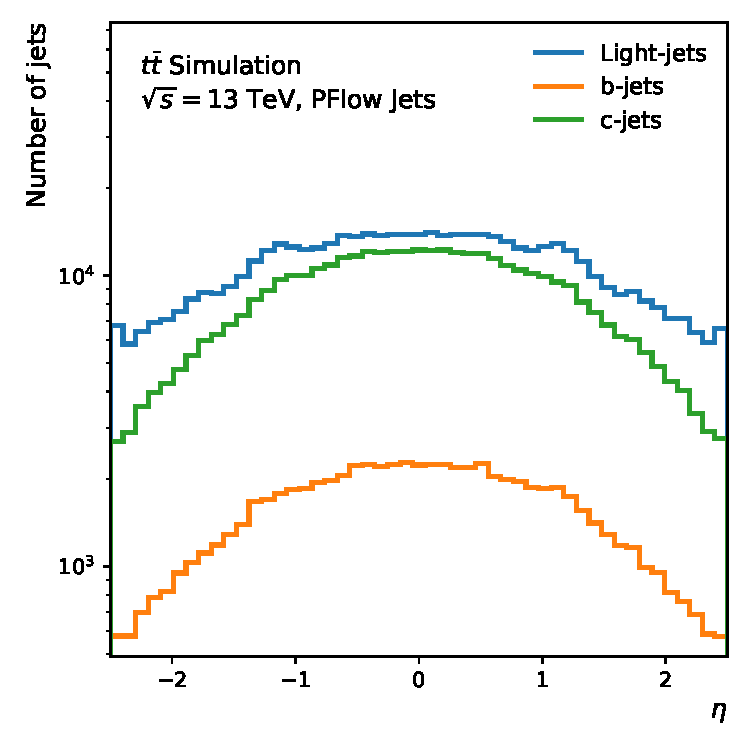
\includegraphics[width=0.45\textwidth]{figures/flavour_tagging/ttbar_0.pdf}
    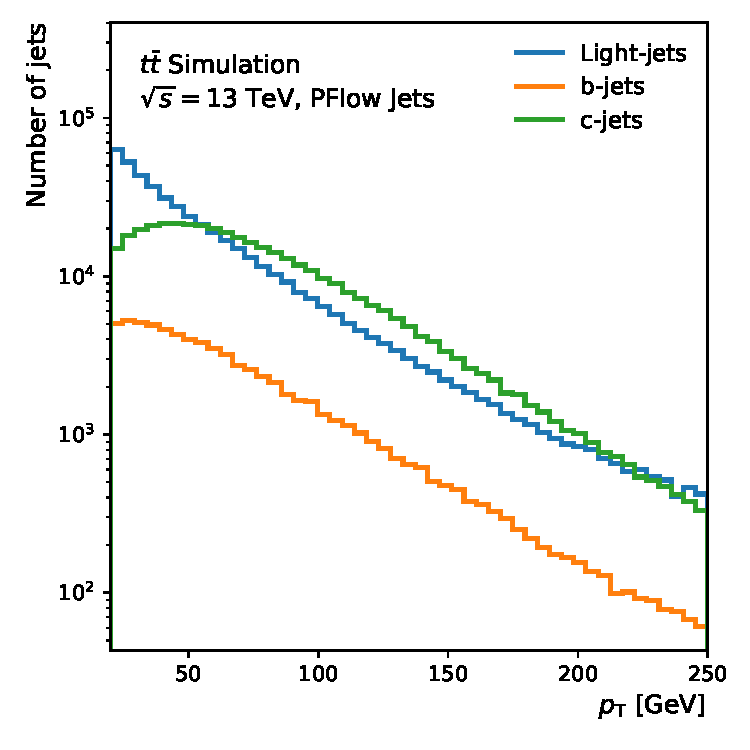
\includegraphics[width=0.45\textwidth]{figures/flavour_tagging/ttbar_1.pdf}
    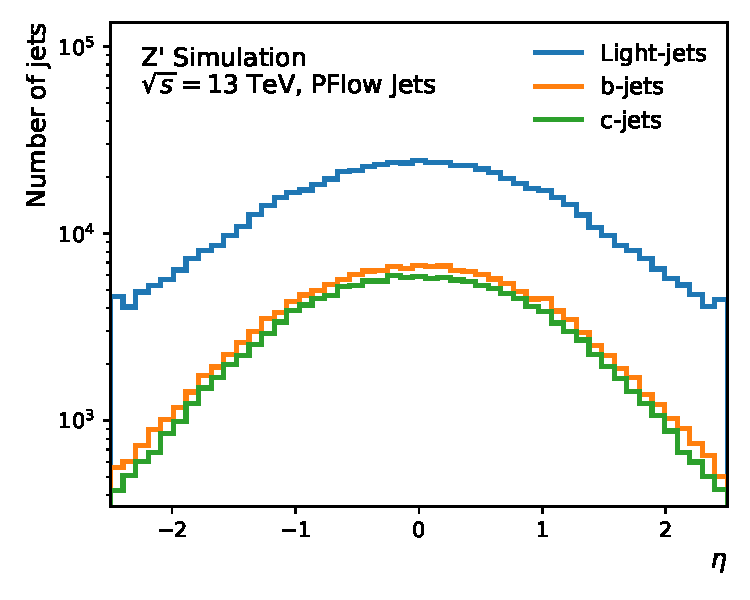
\includegraphics[width=0.45\textwidth]{figures/flavour_tagging/zprime_0.pdf}
    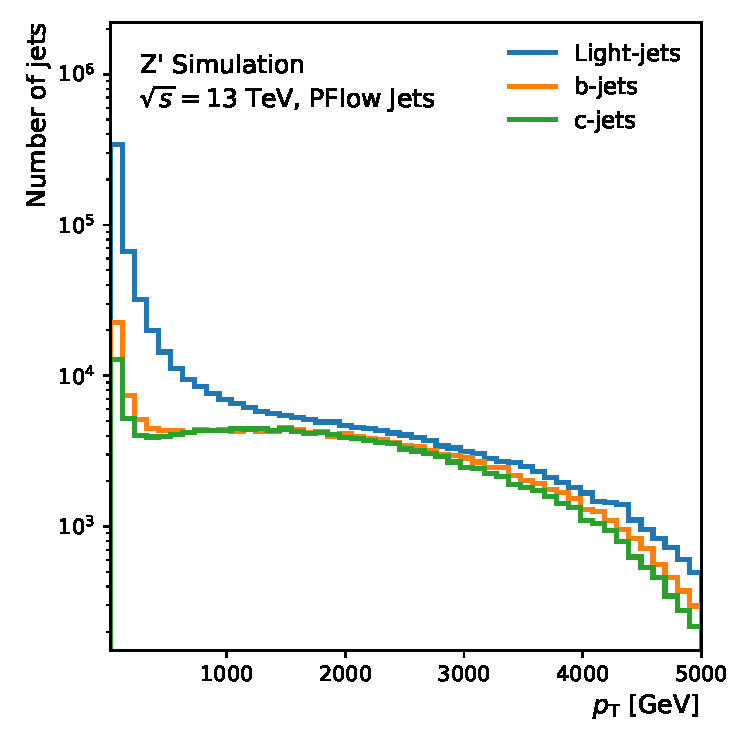
\includegraphics[width=0.45\textwidth]{figures/flavour_tagging/zprime_1.pdf}
    \caption{Original jet $\pt$ (left) and $\eta$ (right) distributions for the $\ttbar$ (top) and $Z'$ (bottom) training datasets. Plots were created using a representative sample.}
    \label{fig:jet_pt_eta}
\end{figure}

\subsection{Monte Carlo Generation}

Simulated proton-proton collisions initiate both datasets at a centre-of-mass energy of $\sqrt{s} = 13~\TeV$.
Hard-scatter events for the $\ttbar$ sample were generated at next-to-leading order using \textsc{PowhegBox v2}~\cite{Powheg1, Powheg2, Powheg3}.
These events were then interfaced with \textsc{Pythia 8.230}~\cite{Pythia8} using the \textsc{A14} tune~\cite{A14} to perform parton showering and hadronization.
For the parton distribution functions, the \textsc{NNPDF3.0NNLO}~\cite{PDF3.0} set was used for matrix element calculations, while the \textsc{NNPDF2.3LO}~\cite{PDF2.3} set was used for showering.
The cut-off scale parameter for the first-gluon-emission $h_{\text{damp}}$ was set to 1.5 times the top quark mass of $m_t = 172.5~\GeV$.
The $Z'$ sample was generated and showered using \textsc{Pythia 8.212} with the \textsc{A14} tune and the \textsc{NNPDF2.3LO} set of parton distribution functions.
The flat mass distribution of the $Z'$ boson was achieved by applying a per-event weight to broaden the natural decay width of the $Z'$ boson.

Decays of $b$- and $c$-hadrons were simulated using the \textsc{EvtGen v1.6.0} package \cite{EvtGen}.
The detector response was performed using the \textsc{Geant4} simulation package~\cite{Geant4} with the ATLAS simulation setup~\cite{ATLASSim}.
Interactions with heavy flavour hadrons and the detector material were not simulated but accounted for in correction factors and systematic uncertainties.
Pileup was modelled by overlaying extra minimum bias events using the \textsc{Pythia 8.160} generator with the \textsc{A3} tune~\cite{A3} and the \textsc{NNPDF2.3LO} parton distribution functions.
These signals are combined with the hard-scatter signals during the digitization step.
In-time pileup was modelled using an average of 40 interactions per bunch crossing, while out-of-time pileup was modelled using bunch crossings before and after the primary interaction.

\subsection{Reconstruction}

The simulation output was reconstructed using the standard ATLAS reconstruction procedure described in \Cref{sec:event_reconstruction}.
In these experiments, the inputs to the model stem from the tracks, and no calibrated physics objects, such as reconstructed photons, electrons, or muons, are used.

Charged particle tracks are required to pass the loose selection criteria~\cite{DL1D} as shown in \Cref{tab:track_loose}.
The primary vertex (PV) is the vertex with the highest sum of squared transverse momenta of the associated tracks.
The impact parameters (IPs) for each track are measured with respect to the PV of the event.
Jets are reconstructed from particle-flow objects~\cite{PFlow} using the anti-$k_t$ algorithm with a radius parameter of $R = 0.4$.
More details are covered in \Cref{sec:particle_flow}.
Tracks are associated with a jet based on the $\Delta R$ separation to the jet axis.
The threshold decreases as a function of the jet $\pt$ to account for the increased collimation of the jet cone, from $\Delta R = 0.45$ at $\pt = 20~\GeV$ to $\Delta R = 0.25$ at $\pt \geq 200~\GeV$.
A track associated with multiple jets is assigned to the jet with the smallest $\Delta R$ separation.

\begin{table}
    \centering
    \begin{tabular}{ll}
        \toprule
        Variable & Requirement \\
        \midrule
        $\pt$ & $> 1~\GeV$ \\
        $d_0$ & $< 3.5~\mm$ \\
        $z_0 \sin \theta$ & $< 5~\mm$ \\
        Number of hits in the SCT & $\geq 8$ \\
        Number of hits shared by other tracks & $\leq 2$ \\
        Number of holes in the SCT & $\leq 3$ \\
        Number of holes in the pixel detector & $\leq 2$ \\
        \bottomrule
    \end{tabular}
    \caption{Loose selection criteria for charged particle tracks~\cite{DL1D}. A hole is defined as a missing hit in a layer where one is expected.}
    \label{tab:track_loose}
\end{table}

\subsection{Truth Labelling}

As with GN1, these networks are trained to perform three complementary tasks.
The primary task is to classify the jet flavour.
The first \textit{auxiliary} task is to predict the origin of each track within the jet. The second \textit{auxiliary} task is to segment the jet: given any two tracks from the same jet, determine if they emerged from the same vertex. Each of these requires defining ground truth labels.

For the primary task, the truth labels of the jets stem from the existence of generator level particles within a $\Delta R$ separation of 0.3.
The jet is associated with the particle with the highest priority within this radius.
The considered particles in order of decreasing priority are, $b$-hadrons, $c$-hadrons, and $\tau$ leptons, which will result in the jet being labelled as a $b$-jet, $c$-jet, $\tau$-jet respectively.
If no such particles are found, the jet is labelled as a light-jet.
We discard $\tau$-jets for this study.

The labels for the track origin are derived by matching the reconstructed track hits to the simulated hits a particle made during the \textsc{Geant4} simulation.
This matching criterion is performed using the~\textit{truth-matching probability} (TMP)~\cite{PerformanceATLASTrack}, this is a ratio of the matched hits to the total number of hits in the track with added factors to account for the varying hit efficiencies of the pixel detector, SCT, and TRT\@.
Each track is associated with the truth particle with the highest TMP\@.
If no truth particle leads to a TMP greater than 0.75, the track is labelled ``Fake'' as it is likely to have been reconstructed from signals produced by multiple overlapping particles.
Once the track is associated with a truth particle, it is classified based on the origin.
The tracks have eight possible classes which are shown in \Cref
{tab:track_labels}.

Finally, the truth vertex labels are binary, indicating whether a pair of tracks emerged from the same secondary vertex within the jet.
The label does not depend on the ordering of the pair, and self-pairs are not considered; thus, for a jet with $N$ tracks, there are $N(N-1)/2$ vertex labels.
The label is set to True if the associated truth particles of each track share an origin within $1~\mm$ of each other.
If one of the tracks is labelled as ``Fake'' or from a pileup interaction, the pair is always labelled False.

\begin{table}
    \centering
    \begin{tabular}{ll}
        \toprule
        Class & Description \\
        \midrule
        1 & From a $b$-hadron decay \\
        2 & From a $c$-hadron decay which itself originated from a $b$-hadron \\
        3 & From a $c$-hadron decay not originating from a $b$-hadron \\
        4 & From a $\tau$-lepton decay \\
        5 & From other secondary decays such as kaons \\
        6 & From the primary vertex \\
        7 & From a pileup $pp$ interaction \\
        8 & A ``Fake'' track from multiple overlapping particles \\
        \bottomrule
    \end{tabular}
    \caption{The eight possible classes for each track based on the origin of the associated truth particle.}
    \label{tab:track_labels}
\end{table}

\subsection{Selection and Sampling}

Jets are required to have $\pt > 20~\GeV$ and $|\eta| < 2.5$ and may not overlap with a generator-level lepton from a $W$ or $Z$ decay.
From the $Z'$ sample, jets must have $\pt > 250~\GeV$ to avoid simulation artefacts.
All jets with $\pt < 60~\GeV$ and $|\eta| < 2.4$ must also pass the tight working point of the JVT algorithm in order to minimize contributions from pileup~\cite{JVT}.

As shown in \Cref{fig:jet_pt_eta}, there is a significant difference between the jet $\pt$ and $\eta$ distributions for the three jet flavours and the two simulated datasets.
This discrepancy would bias the model's training and lead to issues down the line.
Therefore, to mitigate this, the training dataset is resampled with replacement to ensure that the 2D distribution of jet $\pt$ and $\eta$ is identical for the three jet flavours~\cite{AlexThesis}.
After resampling the training set contains a total of 120 million jets split equally between the three jet flavours.
The composition of the training set is around 70\% $\ttbar$ and 30\% $Z'$ events.
The distributions of the jet $\pt$ and $\eta$ for the resampled datasets are shown in \Cref{fig:train_jet_pt_eta}.
During training, 5\% of this was reserved for hold out cross validation.

Two statistically independent test samples were also produced to evaluate the trained models.
After applying the same selection criteria, these test sets contain 1 million $\ttbar$ and $Z'$ jets, respectively.
No resampling was applied to the test datasets.

\begin{figure}
    \centering
    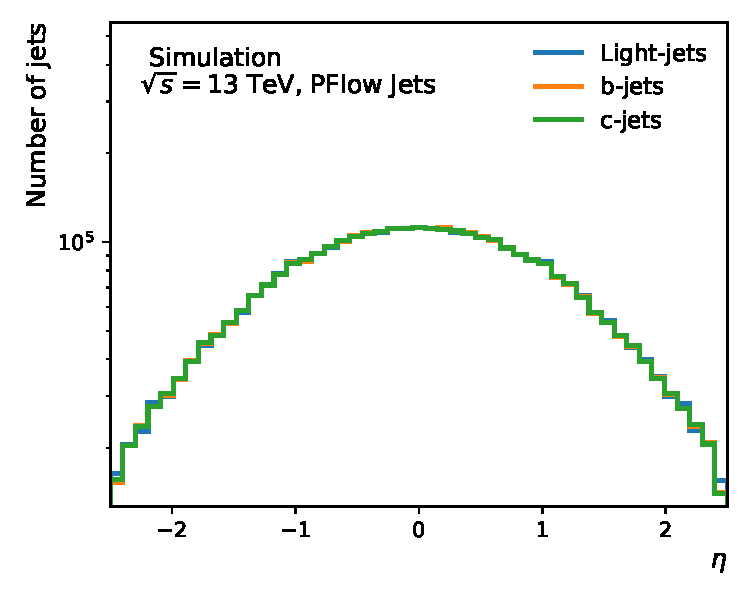
\includegraphics[width=0.45\textwidth]{figures/flavour_tagging/train_0.pdf}
    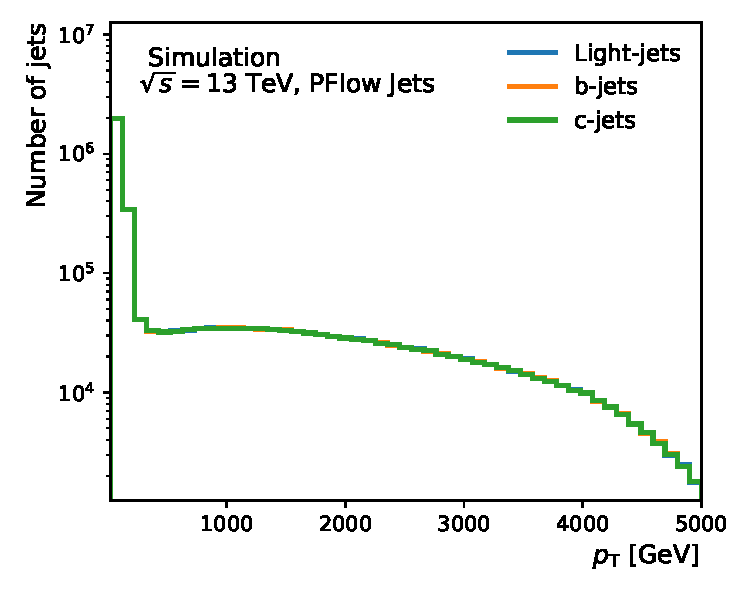
\includegraphics[width=0.45\textwidth]{figures/flavour_tagging/train_1.pdf}
    \caption{Resampled jet $\pt$ (left) and $\eta$ (right) distributions for the training dataset. For these plots only 10M jets were selected as a representative sample.}
    \label{fig:train_jet_pt_eta}
\end{figure}

\subsection{Input Features}

The inputs to all models presented in this chapter are the same as those used in GN1.
They include two kinematic jet variables, $\pt$ and $\eta$, and up to 40 tracks associated with the jet.
Each track is represented by a vector containing 21 features, detailed in \Cref{tab:track_features}.
Almost all $\ttbar$ jets contain less than 40 tracks, but a non-negligible fraction of $Z'$ jets contain more than 40, as shown in \Cref{fig:track_multiplicity}.
For these jets, only the 40 tracks with the highest transverse IP significance $s(d_0)$ are retained.
All features are preprocessed via standardization to have zero mean and unit variance based on the training set statistics.

\begin{figure}
    \centering
    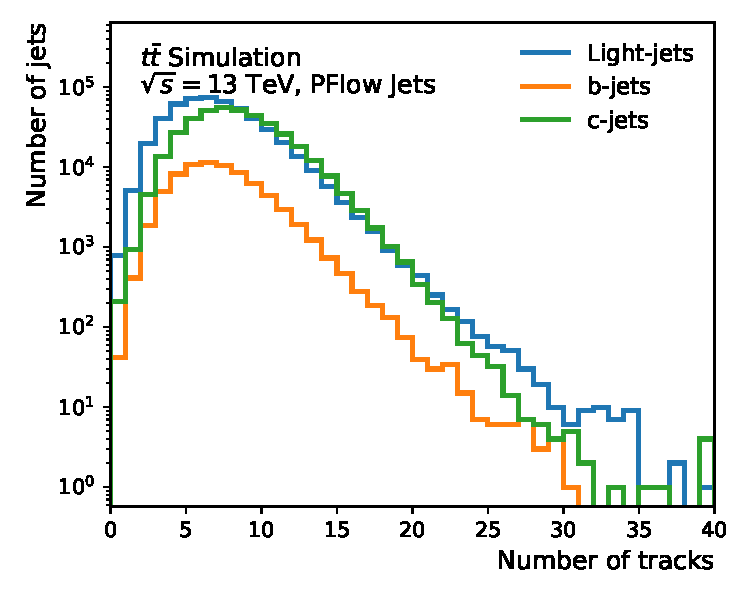
\includegraphics[width=0.45\textwidth]{figures/flavour_tagging/ttbar_2.pdf}
    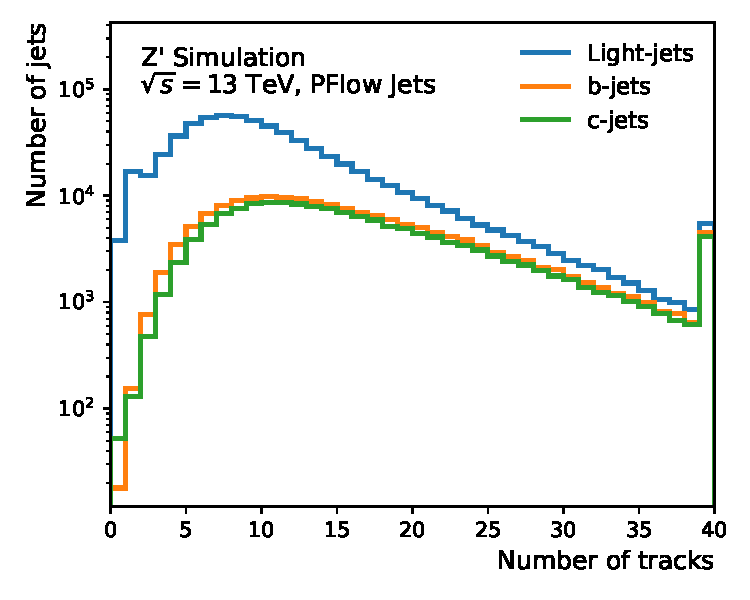
\includegraphics[width=0.45\textwidth]{figures/flavour_tagging/zprime_2.pdf}
    \caption{Original non-resampled number of tracks associated with each jet in the $\ttbar$ (left) and $Z'$ (right) datasets.}
    \label{fig:track_multiplicity}
\end{figure}

\begin{table}[h]
    \centering
    \begin{tabular}{ll}
        \toprule
        \midrule
        \multicolumn{2}{c}{Jet level inputs} \\
        \midrule
        $\pt$ & Jet transverse momentum \\
        $\eta$ & Signed jet pseudorapidity \\
        \midrule
        \midrule
        \multicolumn{2}{c}{Track level inputs} \\
        \midrule
        $q/p$ & Track charge divided by momentum \\
        $\Delta\eta$ & Pseudorapidity of the track relative to the jet $\eta$ \\
        $\Delta\phi$ & Azimuthal angle of the track relative to the jet $\phi$ \\
        $d_0$ & Closest distance from the track to the PV in the longitudinal plane \\
        $z_0 \sin \theta$ & Closest distance from the track to the PV in the transverse plane \\
        $\sigma(q/p)$ & Uncertainty on q/p \\
        $\sigma(\theta)$ & Uncertainty on track polar angle $\theta$ \\
        $\sigma(\phi)$ & Uncertainty on track azimuthal angle $\phi$ \\
        $s(d_0)$ & Lifetime signed transverse IP significance \\
        $s(z_0)$ & Lifetime signed longitudinal IP significance \\
        nPixHits & Number of pixel hits \\
        nSCTHits & Number of SCT hits \\
        nIBLHits & Number of IBL hits \\
        nBLHits & Number of B-layer hits \\
        nIBLShared & Number of shared IBL hits \\
        nIBLSplit & Number of split IBL hits \\
        nPixShared & Number of shared pixel hits \\
        nPixSplit & Number of split pixel hits \\
        nSCTShared & Number of shared SCT hits \\
        nPixHoles & Number of pixel holes \\
        nSCTHoles & Number of SCT holes \\
        \bottomrule
    \end{tabular}
    \caption{Input features for the GNN flavour taggers~\cite{GN1}.}
    \label{tab:track_features}
\end{table}

\section{Model Design}

All the proposed models can be considered as extensions of GN1.
Both Spice and GN++ adhere to a similar framework, but incorporate advancements in message passing techniques and contemporary architectural trends.
The concept of the GN Block, as introduced by~\textcite{RelationalInductiveBiases}, includes features such as persistent edge information, persistent global information, and dedicated node updates.
Furthermore, we explored the transformer architecture, which uses the SDPA to perform message passing.
Other aspects of transformer design, such as PreNorm and residual additive connections, were retrofitted to the GN Block.

GN1 introduced the idea of a monolithic graph neural network which would simultaneously perform jet tagging, track identification, and vertexing matching.
If we frame the input data as a graph, the tracks are the nodes, and the associated jet kinematics are the global attributes.
In this context, there is no explicit graph structure or edge features, although one can include them by deriving attributes from pairs of tracks.
The three training objectives are equivalent to performing a graph-level task, a node-level task, and an edge-level task simultaneously.
Thus, one can think of these models as mappings from the graph structure $(\mathcal{N}, \emptyset, \u) \rightarrow (\mathcal{N}', \mathcal{E}', \u')$, and the loss is calculated on each of the three outputs.

While the edges are featureless, all models treat the graph as fully connected, allowing each node to send and receive messages from all others.
Self-loops are also permitted.
This fully connected approach was found to be beneficial for performance while not significantly increasing the computational cost, as the maximum cardinality of the graph is limited to 40, a relatively low value compared to other graph-based tasks in machine learning.

To compare the information flow within the layers of each of these GNNs, we use the flowcharts in \Cref{fig:gn1_graph}, \Cref{fig:gnpp_graph}, \Cref{fig:gna_graph}, and \Cref{fig:spice_graph}.
These diagrams share similarities with the illustrations of the GN Block \Cref{fig:gn_block} but explicitly display the tensor operations acting on each attribute.
The key for each operation is shown in \Cref{fig:key}.

\begin{figure}[h!]
    \centering
    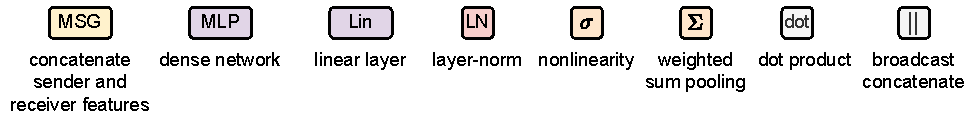
\includegraphics[width=0.99\textwidth]{figures/flavour_tagging/key.pdf}
    \caption{Key for the flowcharts of the GNN operations.}
    \label{fig:key}
\end{figure}

\subsection{GN1}

We first describe the specifics of the GN1 model to better highlight the changes made in GN++ and Spice.
It is worth highlighting that we are comparing to the original GN1 implementation as described in Ref.~\cite{GN1}, as later variants began to adopt more transformer-like features, such as multi-headed attention and multiple projection matrices before the entire shift to Spice/GN2.

The model begins with a track initializer, an MLP that inputs the concatenated track and jet features and outputs a node embedding of size 64.
The embedded node features are then passed through 1 GATv2 layers~\cite{GATv2} to produce a set of updated node features.
The node features are projected within each layer using a learnable square matrix $\W$, which is used to simultaneously calculate the message sent between each pair as well as the message weight using,
\begin{align}
    \vert_{ij} &= \W \x_i, \\
 e_{ij} &= \text{softmax}_i\left(\ba \cdot \relu\left([\W \x_i, \W \x_j]\right)\right).
\end{align}
Here, $\vert_{ij}$ is the message sent from node $i$ to node $j$,
$e_{ij}$ is the weight of that message and $\ba$ is a learnable vector.
A softmax is applied to ensure the total weight of all incoming messages to each node sums to one.
The messages are then aggregated to update the node information across the graph,
\begin{equation}
    \x_j' = \relu\left(\sum_{i} e_{ij} \vert_{ij}\right).
\end{equation}

GN1 uses three of these layers to build its central feature extractor.
The final node features $\{\x_i'\}_{i=1}^{N}$ are then aggregated using a weighted sum to create a pooled graph representation,
\begin{equation}
    \con = \sum_{i} \text{softmax}_i\left(\bias \cdot \x_i'\right) \x_i',
\end{equation}
where $\bias$ is a learnable vector.
The tensor $\con$ is passed through an MLP to produce an output of size 3, which can be used for the graph-level classification task.
For the node-level task, final node features are each concatenated with $\con$ and passed through another MLP with 8 outputs.
For the edge-level task, all possible pairs of nodes are concatenated, not including self-pairs, and passed through a third MLP with a single output.
In total GN1 has 820k trainable parameters with many of them being located in these three output MLPs and the track initializer.
The model was implemented using the PyTorch Geometric library~\cite{PYG}.

A schematic diagram of the GN1 network is shown in \Cref{fig:gn1_graph}.
Some notable limitations of the GN1 model are tied to the usage of GATv2.
These layers reuse the same projection matrix $\W$ to calculate the message content and weight.
These operations could be performed better with specialized layers.
Most notably missing are any strong node updates after the message passing step as framing this in the context of the GN Block means that the node update $\phi^x$ is simply an elementwise ReLU activation function.

\begin{figure}
    \centering
    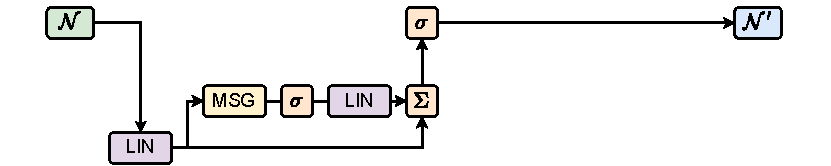
\includegraphics[width=0.99\textwidth]{figures/flavour_tagging/gn1.pdf}
    \caption{Diagram of the operations within a GATv2 layer~\cite{GATv2}}
    \label{fig:gn1_graph}
\end{figure}

\subsection{GN++}

The GN++ model is based on the complete GN Block architecture described in \Cref{sec:gn_block} with the only omission being the lack of a $\rho^{e \to u}$ pooling operation as we found that it was computationally expensive and did not improve performance.
This model is designed to be a more expressive graph network than GN1.
While each layer of GN1 operates on a set, GN++ operates on a graph with fully defined nodes, edges, and global attributes.
We also design GN++ to utilize the standard techniques for training large models.
This model was built using a custom graph library for PyTorch and was explicitly designed to be modular.
Thus, each of the operations within the GN Block could be easily deactivated.
We experimented with several designs.
Our best-performing model uses persistent edge features, persistent global features, layer normalization applied to the inputs of each learnable sub-layer, residual connections around each update, and multi-headed attention.
A diagram of the information flow in a single of these layers is shown in \Cref{fig:gnpp_graph}, and pseudocode is shown in \Cref{alg:gnpp}.

\begin{figure}[h!]
    \centering
    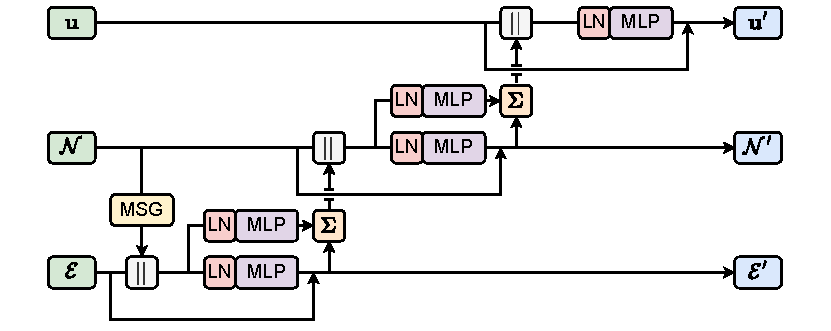
\includegraphics[width=0.99\textwidth]{figures/flavour_tagging/gnpp.pdf}
    \caption{Diagram of the operations within layer of the GN++ tagger.}
    \label{fig:gnpp_graph}
\end{figure}

\begin{algorithm}[h!]
    \caption{The full GN++ block. All weight calculations are followed by a softmax operation and square brackets denote concatenation.}
    \label{alg:gnpp}
    \begin{algorithmic}[1]
        \State \textbf{Input:} Graph attributes $\mathcal{G} = (\mathcal{N}, \mathcal{E}, \u)$
        \State \textbf{Output:} Updated graph attributes $\mathcal{G}' = (\mathcal{N}', \mathcal{E}', \u')$
        \For{each edge $\edge_k$ in $\mathcal{E}$}
            \State $\edge_k' \gets \text{MLP}_e(\lnorm[\edge_k, \x_{s_k}, \x_{r_k}, \u]) + \edge_k$ \Comment{residual update to edge features}
            \State $\w_k \gets \text{MLP}_{e \to x}(\lnorm[\edge_k, \x_{s_k}, \x_{r_k}, \u])$ \Comment{calculate edge weights}
        \EndFor
        \For{each node $\x_i$ in $\mathcal{N}$}
            \State $\mathbf{\bar\edge}_i \gets \sum_{k: r_k = i} \w_k \edge_k'$ \Comment{attention pool edges}
            \State $\x_i' \gets \text{MLP}_v(\lnorm[\mathbf{\bar\edge}_i, \x_i, \u]) + \x_i$ \Comment{residual update to node features}
            \State $\w_i \gets \text{MLP}_{x \to u}(\lnorm[\mathbf{\bar\edge}_i, \x_i, \u])$ \Comment{calculate node weights}
        \EndFor
        \State $\mathbf{\bar{x}} \gets \sum_{i} \w_i \x_i'$ \Comment{attention pool nodes}
        \State $\u' \gets \text{MLP}_u(\lnorm[\mathbf{\bar{x}}, \u]) + \u_i$ \Comment{residual update to global attributes}
    \end{algorithmic}
\end{algorithm}

In a single layer, there are 5 MLPs: 3 to perform the updates $\phi^x$, $\phi^e$, and $\phi^u$, and two to calculate the attention weights for the $\rho^{e \to x}$ and $\rho^{x \to u}$ steps.
Multi-headed attention is achieved by having multiple outputs for the $\rho^{e \to x}$ and $\rho^{x \to u}$ MLPs, and each is softmaxed separately.
We fin the best performance with four attention heads.
All updates are additive residuals, and the weights of the final layer of each update MLP are initialized with zeros.
All MLPs have a single hidden layer which doubles the embedding dimension, applies the LeaklyReLU activation, and projects back to the original.

We use a basic linear projection for the track initializer instead of a full MLP\@.
Edges and global information are treated as empty for the first layer, after which they are initialized to have the same dimension as the node features.
The three networks for the graph, node, and edge tasks are no longer required, as the GN Block already has outputs for each level.
We simply change the output dimension of the final update MLPs to match the required dimension of each task.
The residual connections in this final GN Block are each passed through a linear resizing layer to match the output dimension.
We use 5 graph layers in total, each with half the embedding dimension of GN1, to roughly have the same number of parameters.
The GN++ model has 780k trainable parameters.

As each of these operations is optional, we can easily deactivate them to investigate their impact on performance.
The minimal model, which we call GNA, is shown in \Cref{fig:gna_graph}, and it is close to but not exactly the same as GN1.
This provides us a good baseline to slowly add complexity to the model and investigate the impact of each operation.

\begin{figure}[h!]
    \centering
    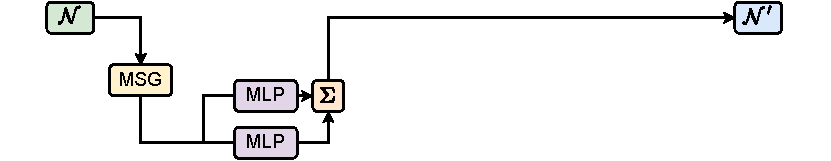
\includegraphics[width=0.99\textwidth]{figures/flavour_tagging/gna.pdf}
    \caption{Diagram of the operations within one layer of the GNA tagger.}
    \label{fig:gna_graph}
\end{figure}

\subsection{Spice}

The Spice model is based on the transformer-encoder architecture described in \Cref{sec:transformer_variants}.
As a transformer, each layer does not produce or retain edge features, and message passing is performed using multi-headed self-attention.

We find the best performance using four attention heads.
Like GN++, the model is equipped with strong node updates in the form of MLPs, which double the hidden dimension of the nodes.
The information flow diagram is shown in \Cref{fig:spice_graph}.

To construct the pooled graph representation $\con$, we use three CA Blocks with four attention heads to send messages from each track onto a single learnable class token~\cite{GoingDeeper}.
This process allows the model to decide on a jet-by-jet basis what information to request from the tracks to assist with classification.
Like GN1, three separate MLPs perform the graph-, node-, and edge-level tasks.
These three MLPs and the track initializer are much smaller than the ones used in GN1, which reduces the number of parameters in the model.

Spice's primary hyperparameters are the embedding dimension and the number of TE Blocks, which vary to investigate the tagger's scaling capabilities.
The model was implemented using standard PyTorch operations and is thus conceptually easier to work with than GN++ and GN1.

\begin{figure}[h!]
    \centering
    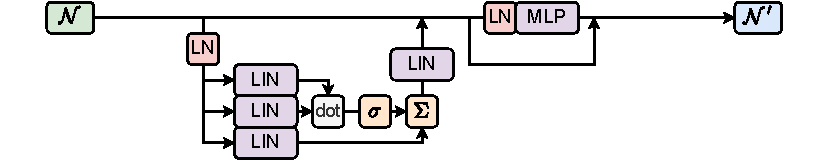
\includegraphics[width=0.99\textwidth]{figures/flavour_tagging/spice.pdf}
    \caption{Diagram of the operations within one TE layer of the Spice tagger. The multiple attention heads are not shown for clarity.}
    \label{fig:spice_graph}
\end{figure}

\section{Training}

We reuse the same training loss as GN1, involving a weighted sum of three loss terms,
\begin{equation}
  \mathcal{L} = \mathcal{L}_{\text{graph}} + \alpha \mathcal{L}_{\text{node}} + \beta \mathcal{L}_{\text{edge}}.
\end{equation}
The graph loss $\mathcal{L}_{\text{graph}}$ is a cross-entropy loss between the predicted jet flavour and the ground truth.
The node loss $\mathcal{L}_{\text{node}}$ is calculated similarly but for the track origin task and averaged over all tracks in the jet.
The edge loss $\mathcal{L}_{\text{edge}}$ is calculated using a binary cross entropy between the predicted vertex label and the ground truth.
These additional loss terms help steer the model to learn jet representations linked to fundamental physics related to the jet's flavour.
By predicting the true origin of each track and the vertex compatibility of each track-pair the model is actively looking for displaced vertices and thus heavy flavour decays.
These auxiliary training objectives, viewed as ``stepping stones''~\cite{GN1} on the way to determining the flavour of the jet.

Before averaging across the batch, the auxiliary loss terms are multiplied by a per sample weight.
The node task is weighted by the inverse frequency of each category in \Cref{tab:track_labels} found in the training set to account for class imbalance.
The weight for each pair of tracks in the edge task is set to two if the track pair is from a $b$- or $c$-hadron decay and one otherwise.
This reweighting forces the model to focus on heavy flavour vertices, which are more significant for flavour tagging.
No balancing is required for $\mathcal{L}_{\text{graph}}$ due to the resampling of the training set.
Averaging over all jets in the batch does mean that jets with more tracks contribute more to the gradients due to more terms in the track and edge loss, but we found this effect to be minimal.

For the main models, we keep the same loss coefficients as GN1, $\alpha = 0.5$ and $\beta = 1.5$.
We also run ablation studies where $\alpha$ and $\beta$ are set to zero to determine the effect of the auxiliary tasks on the model's flavour tagging performance.

The training configuration for all models was as follows.
The batch size was set to 1024, and the learning rate followed a cyclic schedule, repeating every five epochs.
The minimum learning rate was set to $1.0 \times 10^{-5}$ and the maximum to $5.0 \times 10^{-4}$.
We found that the warm-up period was necessary to prevent the model from diverging.
We used the AdamW~\cite{AdamW} optimizer with a $1.0 \times 10^{-4}$ weight decay.
The training was performed for a maximum of 50 epochs, and the checkpoint with the lowest validation loss was saved for evaluation.
Gradient clipping was applied with a maximum norm of 10.

\section{Results}

We can turn models into binary classifiers using a combination of the three outputs.

into a single $b$-tagging score we use the following formula,
\begin{equation}
    D_b = \log\frac{p_b}{(1-f_c)p_l + f_c p_c},
\end{equation}
where $p_b$, $p_c$, and $p_l$ are the probabilities of the jet being a $b$-, $c$-, and light-jet respectively, and $f_c$ is a free parameter that provides a trade-off between $c$- and light-jet rejection.
The choice of $f_c$ is arbitrary and in GN1 it is set to $0.05$, but for our models we found a better balance at $0.02$.
This procedure may also be used to construct a $c$-tagging score $D_c$ with an equivalent $f_b$ parameter.
We set $f_b = 0.2$ for the $c$-tagging scores, matching GN1.

\newcommand{\bnom}{\epsilon_b^{70}}
\newcommand{\cnom}{\epsilon_c^{25}}
With the scores defined, the performance of the models is quantified quantified by the rejection rate $r_a$ for a specific background $a$, measured at fixed signal efficiency $\epsilon_s$.
The background rejection is defined as the reciprocal of the background efficiency $r_a = \sfrac{1}{\epsilon_a}$.
Specific signal efficiencies are labelled as working points (WPs) and are chosen to match the requirements of an analysis.
Standard WPs for $b$-tagging algorithms in ATLAS are at 60\%, 70\%, 77\%, and 85\%, while the WPs for $c$-tagging are considerably lower, with a WP of 25\% being a common choice.
For brevity, we label the 70\% WP as the nominal WP for $b$-tagging $\bnom$ and the 25\% WP as the nominal WP for $c$-tagging $\cnom$.
Thus to better compare the models, we use receiver operating characteristic (ROC) curves, allowing us to measure the performance of the model at all possible operating points.

The performance of all models is evaluated separately using the two test datasets.
We also individually evaluate the $b$-tagging and $c$-tagging scores.

\subsection{Graph Network Ablation Studies}

In order to test if each of the proposed changes to the graph network to move from GN1 to GN++ are beneficial we perform a grid search over each of the features in \Cref{tab:gnpp_grid}.
The two extremes are the minimal model, GNA which has features deactivated and is similar in design to GN1, and the maximal model GN++, which has all of features activated.
For this section only we limit the training to 5 epochs to reduce the computational cost.

To capture overall trends on the inclusion of these features we can use the $\mathcal{L}_{\text{graph}}$ as measured on the test set.
This is shown in the violin plots of \Cref{fig:violin} which can capture first order effects.
The secondary effects on feature importance can be analysed by training a random forest model to predict the minimum validation $\mathcal{L}_{\text{graph}}$, using the feature activations as input.
To assess the impact of individual features, the performance of the forest can be evaluated after permuting the specific feature column within the dataset.
The results of this analysis are shown in \Cref{tab:feature_importance}.

Notably, all features are beneficial and the best performance was achieved by the maximal model GN++.
The results from the importance studies show that the most crucial feature is the use of persistent edge information by a wide margin.
This is followed by the stronger node updates using MLPs.
The least significant features are the use of PreNorm and residual connections and the latter was only beneficial if combined with node feed-forward updates.
In addition, these features are designed to stabilize the training of deep models, and as we limit ourselves to only 5 layers to match GN1, the benefits are less pronounced.
Persistent global information was not significant, as we are operating on fully connected graphs, therefore long range interactions are already captured by the message passing.

\begin{figure}[ht]
    \centering
    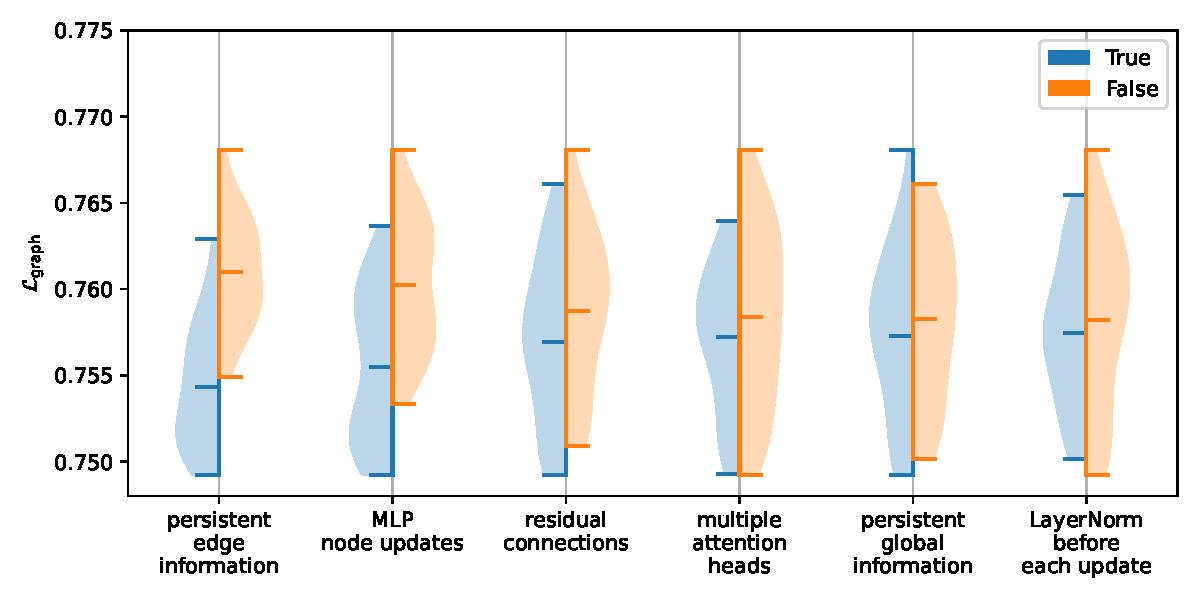
\includegraphics[width=0.99\textwidth]{figures/flavour_tagging/violin.pdf}
    \caption{Violin plots showing the distribution of $\mathcal{L}_{\text{graph}}$ measured on the validation set. Each group represents the activation of a specific graph network feature.}
    \label{fig:violin}
\end{figure}

We further investigate the ablation studies using the $b$-tagging performance on the $\ttbar$ test sample.
For each feature we compare four models, GNA, GNA with the feature activated, GN++, and GN++ with the feature deactivated.
The results for the four most important features are shown in \Cref{fig:ablation}.
For this sample the GN++ tagger is the best performing model, with around 25\% increase over GNA in both light and $c$-jet rejection at $\bnom$.
At the higher efficiency WP of 85\% the improvement drops to around 20\% and 15\% for light and $c$-jets respectively.
Interestingly, the persistent edge information seems to be such a crucial feature that activating only this feature results in a more performant tagger than the one with all others.
Node updates using MLPs barely improves the performance of the model when applied alone as we observed training to be slow and unstable.
However, when combined the other features which assist in stabilizing the training, the performance is significantly improved.

\begin{figure}[ht]
    \centering
    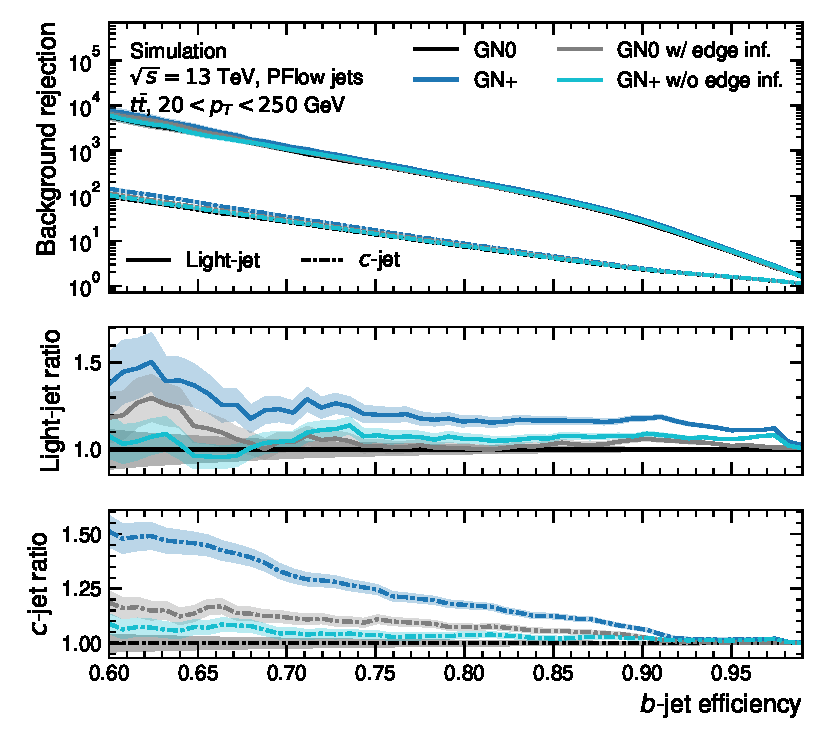
\includegraphics[width=0.49\textwidth]{figures/flavour_tagging/b_roc_ttbar_edge.pdf}
    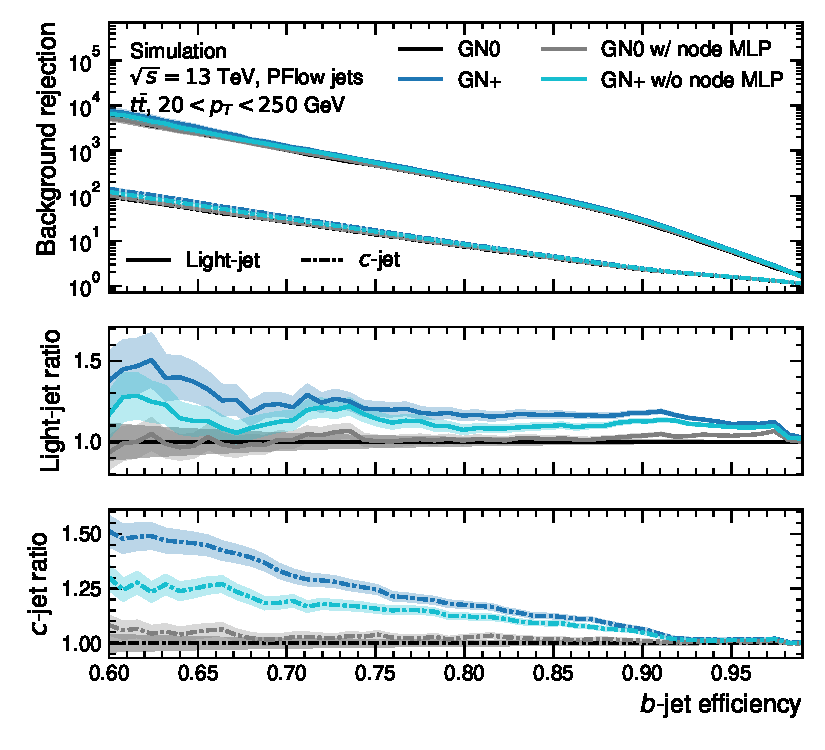
\includegraphics[width=0.49\textwidth]{figures/flavour_tagging/b_roc_ttbar_node.pdf}
    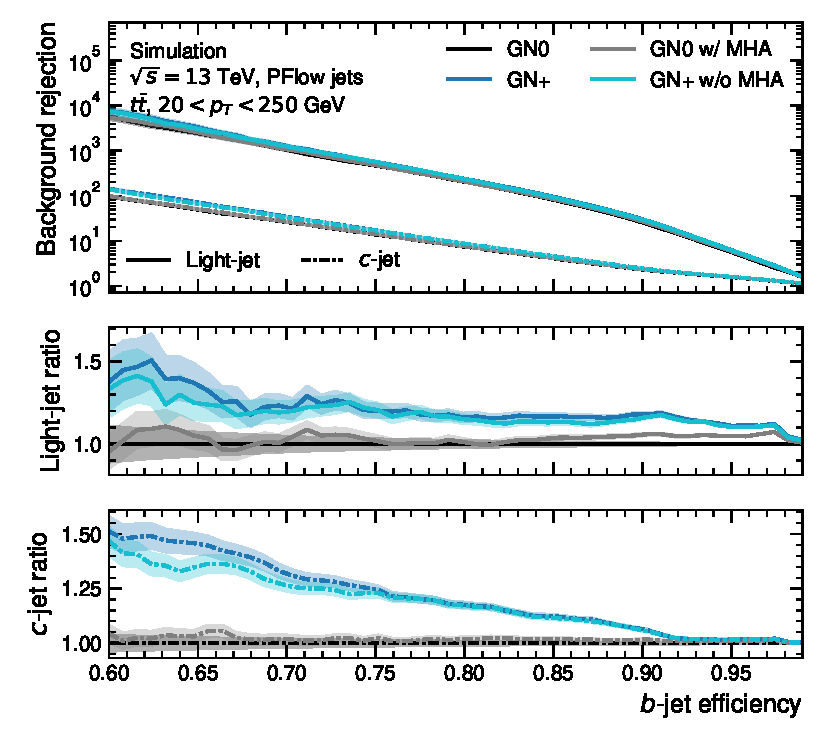
\includegraphics[width=0.49\textwidth]{figures/flavour_tagging/b_roc_ttbar_mha.pdf}
    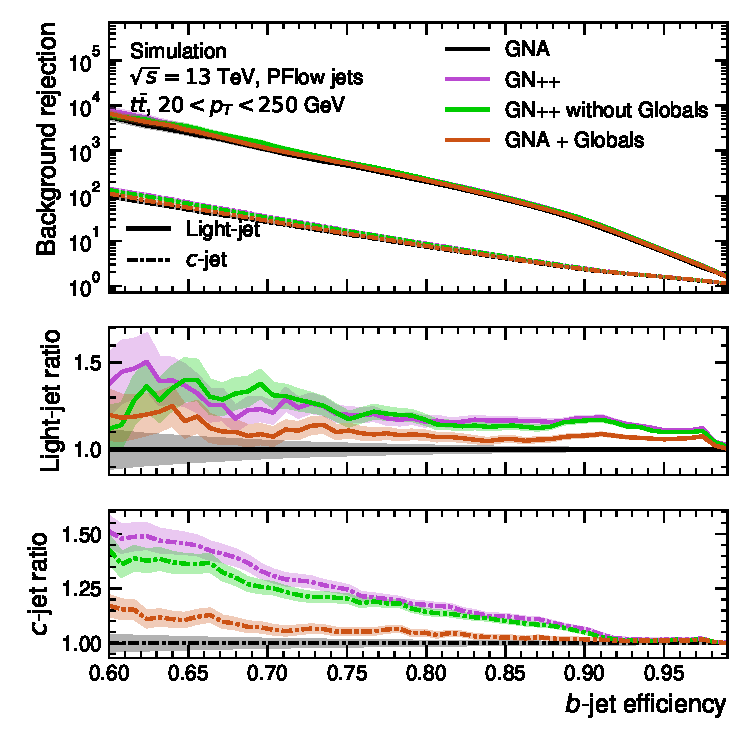
\includegraphics[width=0.49\textwidth]{figures/flavour_tagging/b_roc_ttbar_pg.pdf}
    \caption{ROC curves for the $b$-tagging scores for $\ttbar$ jets with $20 < \pt < 250~\GeV$ for the ablation studies.
    From top-left clockwise the tested features are persistent edge information, nodewise feed-forward updates, multi-headed attention, and persistent global information. The rejection values are calculated separately for light- and $c$-jets. The bottom two panels in each plot show the ratio of these rejection values to the GNA tagger. The error bands show binomial uncertainties. The left plots show the effect of activating persistent edge information in the graph network and the right plots show the effect of activating nodewise feed-forward updates.}
    \label{fig:ablation}
\end{figure}

\begin{table}
    \centering
    \begin{tabular}{lr}
        \toprule
        Feature & Importance \\
        \midrule
        Persistent edge information & 0.51 \\
        Nodewise feed-forward updates & 0.29 \\
        Multi-headed attention & 0.06 \\
        Persistent global information & 0.05 \\
        PreNorm & 0.05 \\
        Residual connections & 0.03 \\
        \bottomrule
    \end{tabular}
    \caption{Feature importance for the graph network ablation studies. The scores are normalized to sum to 1.}
    \label{tab:feature_importance}
\end{table}

\subsection{Tagging Performance}

We look at the performance of both $b$- and $c$-tagging scores for the $\ttbar$ and $Z'$ samples.
We use the ROC curves to compare the performance of the models at all possible operating points, but we also show specific values for the 70\% WP for $b$-tagging and the 25\% WP for $c$-tagging in \Cref{tab:comparison}.


To ensure a fair comparison, we introduce models of various sizes, making sure to have some with roughly the same number of trainable parameters as GN1.
The GN++ and GN1 models already have roughly equivalent sizes, and thus we design a Spice variant with approximately 800k.
This model has 7 TE Blocks and an embedding dimension of 64.
We then investigate how these models scale by introducing two new transformers, Spice-large and Spice-huge.
Both use the same number of layers, but Spice-large has an embedding dimension of 128 and Spice-huge has an embedding dimension of 256\footnote{Note that the FFN within each block always double the embedding dimension.}.
These correspond to 1.4M and 4.2M trainable parameters respectively.
We also introduce GN++large which also has an embedding dimension of 128, leading to 1.6M trainable parameters.

\subsection{Comparison to GN1}

The results for the $\ttbar$ sample are shown in \Cref{fig:ttbar_roc}.
Both new models of equivalent size to GN1 outperform it for $\epsilon_S<90\%$.
For $b$-tagging at $\bnom$, Spice offers a 47\% improvement in light-jet rejection and 38\% improvement in $c$-jet rejection over GN1.
The larger models further increase this performance gain, with Spice-huge offering a 73\% improvement in light-jet rejection and 63\% improvement in $c$-jet rejection.
For $c$-tagging, most of the performance improvement is
found at much lower signal efficiencies.
At the $\cnom$, Spice improves over GN1 by 16\% in $b$-jet rejection and 27\% in light-jet rejection.
It is interesting that Spice is consistently better than GN++ for both $b$- and $c$-tagging on this dataset, as it lacks the feature determined to be the most important in the ablation studies, the persistent edge information.
However, these models are trained for 10 times longer than the ablation studies, so it is possible that the transformer based model is able to learn the same information in a more efficient manner.
For $c$-tagging, once again the most performant model is Spice-huge, which is able to achieve a 26\% $b$-jet rejection improvement and 50\% light-jet rejection improvement over GN1 at $\cnom$.

The results for the much higher $\pt$ $Z'$ sample are shown in \Cref{fig:zprime_roc}.
All models once again outperform GN1.
For the smaller networks GN++ provides higher rejection rates than Spice.
These jets have an order of magnitude higher $\pt$ than the $\ttbar$ jets, and the GN++ model seems to be better suited for this data type.
However, by scaling the models, Spice-large is easily able to outperform GN++ and even GN++large.
It achieves and improvement over GN1 of 25\% in light-jet rejection and 12\% in $b$-jet rejection at $\bnom$.
In $c$-tagging, Spice-large is able to achieve a 27\% improvement in $b$-jet rejection and 22\% improvement in light-jet rejection at $\cnom$.

\begin{figure}[ht]
    \centering
    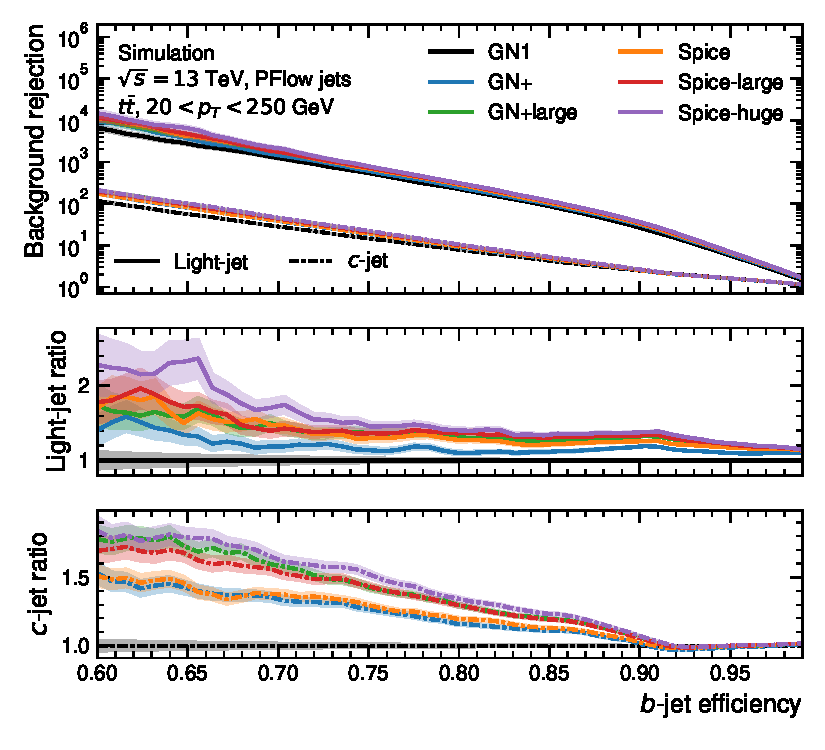
\includegraphics[width=0.49\textwidth]{figures/flavour_tagging/b_roc_ttbar_large.pdf}
    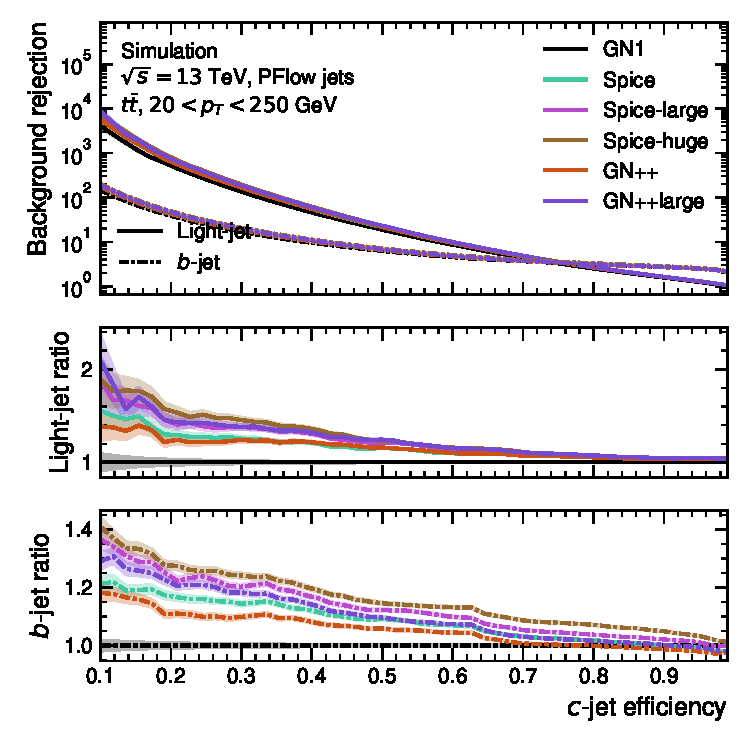
\includegraphics[width=0.49\textwidth]{figures/flavour_tagging/c_roc_ttbar_large.pdf}
    \caption{ROC curves for the $b$-tagging scores (left) and $c$-tagging scores (right) for $\ttbar$ jets with $20 < \pt < 250~\GeV$. The rejection values are calculated separately for each background type. The bottom two panels show the ratio of these rejection values to the GN1 tagger. Error bands are derived from binomial uncertainties.}
    \label{fig:ttbar_roc}
\end{figure}

\begin{figure}[ht]
    \centering
    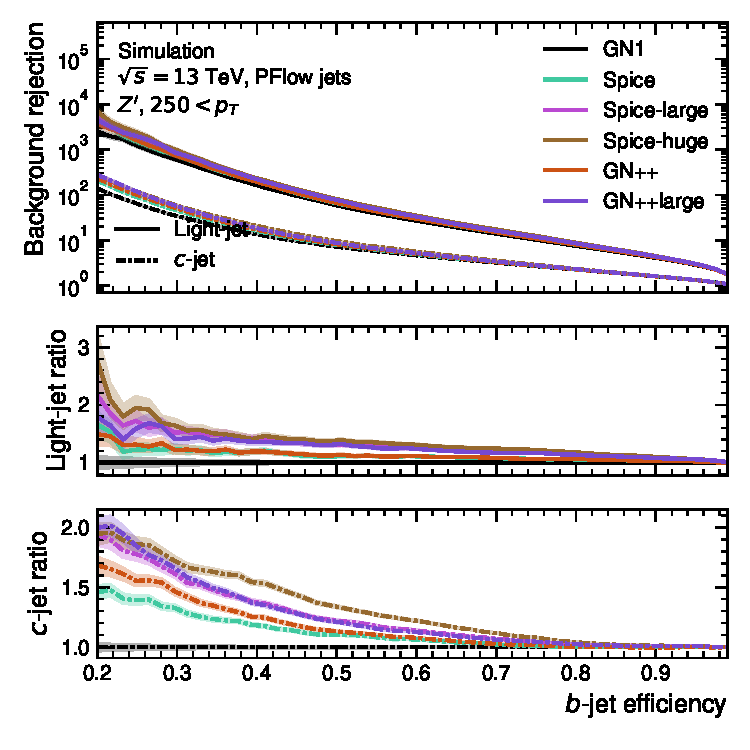
\includegraphics[width=0.49\textwidth]{figures/flavour_tagging/b_roc_zprime_large.pdf}
    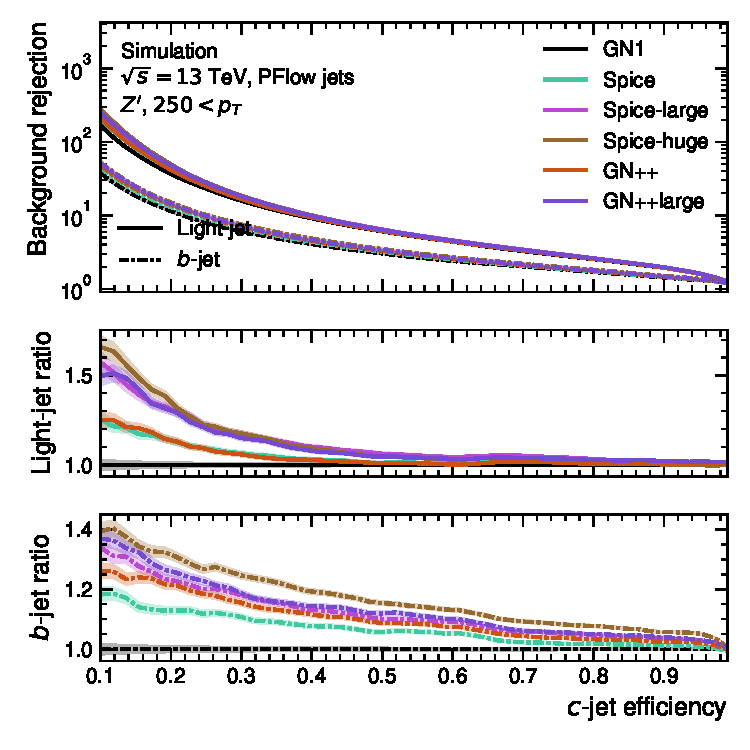
\includegraphics[width=0.49\textwidth]{figures/flavour_tagging/c_roc_zprime_large.pdf}
    \caption{ROC curves for the $b$-tagging scores (left) and $c$-tagging scores (right) for $Z'$ jets with $\pt > 250~\GeV$. The rejection values are calculated separately for each background type. The bottom two panels show the ratio of these rejection values to the GN1 tagger. Error bands are derived from binomial uncertainties.}
    \label{fig:zprime_roc}
\end{figure}

\newcommand{\alen}{\hskip 35pt}
\newcommand{\blen}{\hskip 25pt}
\begin{table}[ht]
    \centering
    \begin{tabular}{l@{\alen}cc@{\blen}cc@{\alen}cc@{\blen}cc}
        \toprule
        & \multicolumn{4}{c@{\alen}}{$\ttbar$} & \multicolumn{4}{c}{$Z'$} \\
        & \multicolumn{2}{c@{\blen}}{$\bnom$} & \multicolumn{2}{c@{\alen}}{$\cnom$}
        & \multicolumn{2}{c@{\blen}}{$\bnom$} & \multicolumn{2}{c}{$\cnom$} \\
        & $r_B^c$ & $r_B^l$ & $r_B^b$ & $r_B^l$ & $r_B^c$ & $r_B^l$ & $r_B^b$ & $r_B^l$ \\
        \midrule
        Spice & 38 & 47 & 16 & 27 & 2 & 8 & 12 & 9 \\
        Spice-large & 54 & 41 & 23 & 38 & 7 & 21 & 20 & \textbf{22} \\
        Spice-huge & \textbf{63} & \textbf{73} & \textbf{26} & \textbf{50} & \textbf{12} & \textbf{25} & \textbf{27} & \textbf{22} \\
        GN++ & 34 & 19 & 10 & 22 & 3 & 8 & 18 & 9 \\
        GN++large & 59 & 46 & 21 & 42 & 6 & 17 & 23 & 21 \\
        \bottomrule
    \end{tabular}
    \caption{The percentage improvement in background rejection rates for the different models with respect to GN1 at the $\bnom = 70\%$ $b$-tagging and $\cnom = 25\%$ $c$-tagging working points using the $\ttbar$ and $Z'$ test datasets. The rejection rates are measured for the light-jet background $r_B^l$, the $c$-jet background $r_B^c$, and the $b$-jet background $r_B^b$.}
    \label{tab:comparison}
\end{table}

\subsection{Auxiliary Task Ablation Studies}

We also investigated if the model still benefits from the two extra auxiliary tasks that were highly beneficial to GN1.
For this we used the Spice-large model, and trained three models, setting $\alpha$, $\beta$, and both to zero.
The results are shown in \Cref{fig:auxiliary} and show that while not as crucial as in GN1, the auxiliary tasks still provide a marginal performance boost on average.
This is most notable for high $\pt$ jets, as shown by the $Z'$ sample.
There are however a couple of specific cases where the auxiliary tasks are detrimental to the performance of the model.
For high signal efficiencies in $c$-tagging, $\approx 80\%$, on the $\ttbar$ sample the model with no vertex task performs around 2\% better than the model with all tasks.
However, this improvement is not significant and it is in a region not typically used in analyses.
Therefore, we conclude that the auxiliary tasks are still beneficial to the model.

\begin{figure}[ht]
    \centering
    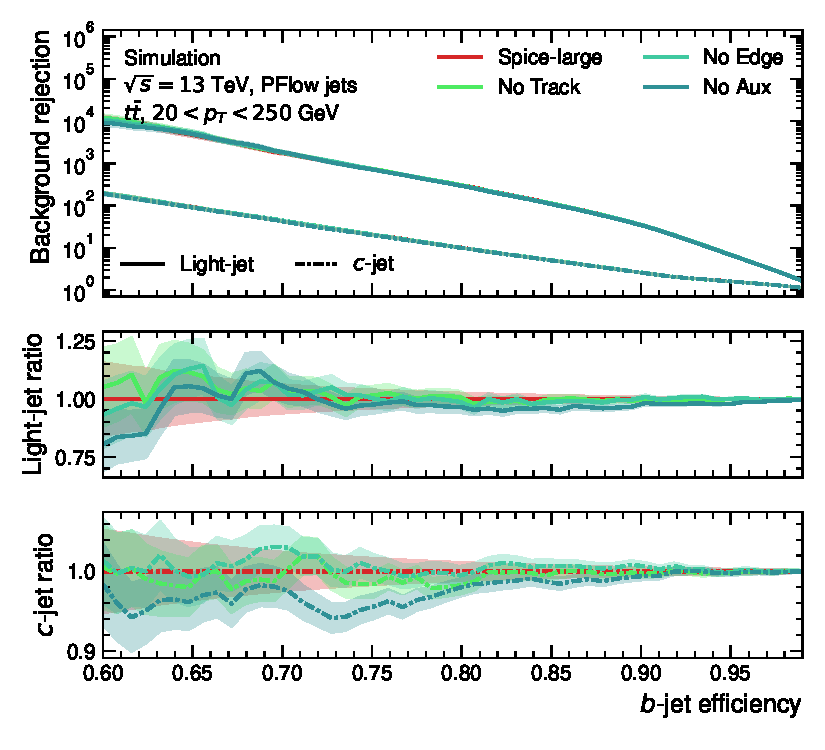
\includegraphics[width=0.49\textwidth]{figures/flavour_tagging/b_roc_ttbar_aux.pdf}
    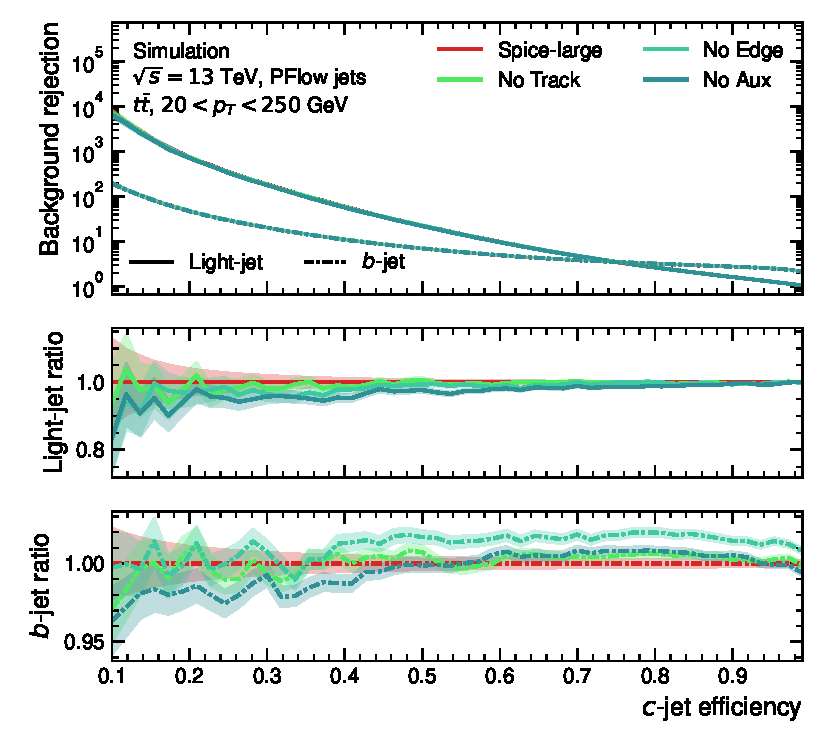
\includegraphics[width=0.49\textwidth]{figures/flavour_tagging/c_roc_ttbar_aux.pdf}
    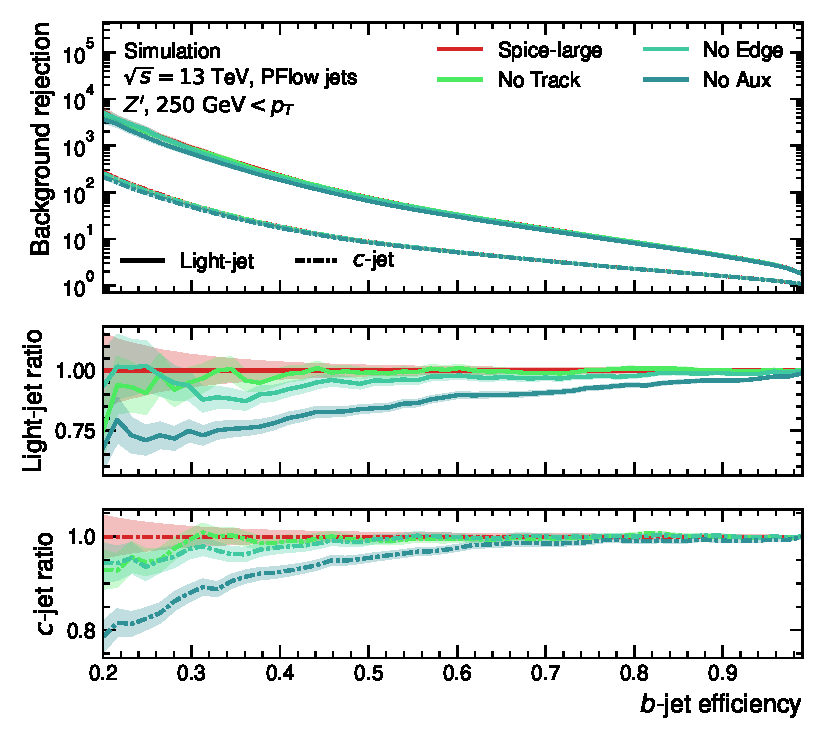
\includegraphics[width=0.49\textwidth]{figures/flavour_tagging/b_roc_zprime_aux.pdf}
    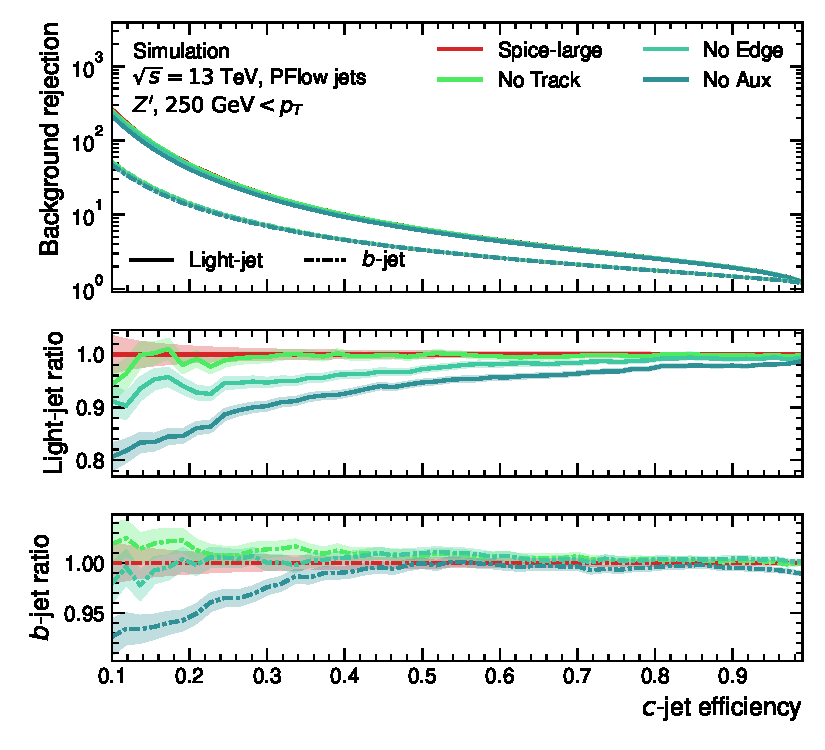
\includegraphics[width=0.49\textwidth]{figures/flavour_tagging/c_roc_zprime_aux.pdf}
    \caption{ROC curves for the $b$-tagging scores (left) and $c$-tagging scores (right) for $\ttbar$ jets with $20 < \pt < 250~\GeV$ (top) and $Z'$ jets with $\pt > 250~\GeV$ (bottom). The rejection values are calculated separately for each background type. The bottom two panels show the ratio of these rejection values to the Spice-large tagger. Error bands are derived from binomial uncertainties.}
    \label{fig:auxiliary}
\end{figure}


\subsubsection{Computational Cost}

Key to the practicality of these models is the computational cost associated with running inference on them.
The GPU and CPU times are shown in \Cref{tab:inference}.
The GPU times are relevant for training the model, and it highlights the ease at which the models can be produced.
When running the taggers for offline analysis, they will be exported via ONNX runtime and run on the CPU\@.
The GN++ models are the slowest to run on both the CPU and GPU\@.
This is likely due to the inefficient implementation of the graph layers in the custom graph library.
This is in contrast to the transformer based models which barely increase in inference time when running on the GPU as so many of the operations are basic matrix multiplications and thus highly parallelized.
Even though the expressivity of a single GN++ layer is theoretically much higher than a single transformer layer, the efficiency of the latter allows it to out-scale the former.
Therein lies the strength of the transformer architecture.
There are potentially many more expressive and smarter graph network designs that posses stronger inductive biases, but the efficiency of the transformer architecture means that simply by scaling the model, it can outperform them.

It is also worth commenting on the ease at which these models can be exported using ONNX runtime.
For both GN1 and GN++, significant effort was spent creating adaptation functions to convert the PyTorch Geometric layers, or the layers from the custom graph library, into ONNX compatible layers.
Each time a new layer was designed, it required new adaptation functions.
In contrast, the transformer model uses standard matrix operations, and thus can be exported directly to ONNX without any additional work.

\begin{table}
    \centering
    \begin{tabular}{lrrr}
        \toprule
        Model & Parameters & GPU Time (ms) & CPU Time (ms) \\
        \midrule
        GN1 & 820k & 0.06 & 1.4 \\
        GN++ & 780k & 0.50 & 23.0 \\
        GN++large & 1.6M & 0.90 & 59.0 \\
        Spice & 800k & 0.03 & 1.5 \\
        Spice-large & 1.4M & 0.05 & 4.4 \\
        Spice-huge & 4.2M & 0.08 & 7.3 \\
        \bottomrule
    \end{tabular}
    \caption{Inference times for the different models on a CPU (AMD EPYC 7742) and GPU (NVIDIA 3090). The CPU times were measured using ONNX exported versions of the models.}
    \label{tab:inference}
\end{table}

\section{GN2 Tagger}

The Salt model was adapted into the new GN2 tagger which is being developed in the Salt~\cite{Salt} framework and is actively being used by the ATLAS Collaboration.

Several and architectural changes were made to the model, differentiating it from the Spice.
There are now 8 TE Blocks, each with an embedding dimension of 192 and a FFN hidden dimension of 256.
This results in a model with 1.5M trainable parameters.
Eight attention heads are used and during training dropout is applied to the attention weights with a drop probability of 0.1.
The three class attention operations were also replaced with a single global attention layer for calculating the pooled graph representation.
The model is trained using a single learning rate cycle which lasts for 40 epochs with a maximal learning rate of $5.0 \times 10^{-4}$.
The training set has also been expanded 192M jets.

GN2 marks a significant improvement over the previous flavour tagging models, as shown in \Cref{fig:ftag_better}, covering over four times greater background rejection $70\%$ $b$-tagging efficiency on $\ttbar$ jets compared to DL1, the tagger used only a few years ago.
Compared to GN1 the improvements are around 50-80\%.

\begin{figure}
    \centering
    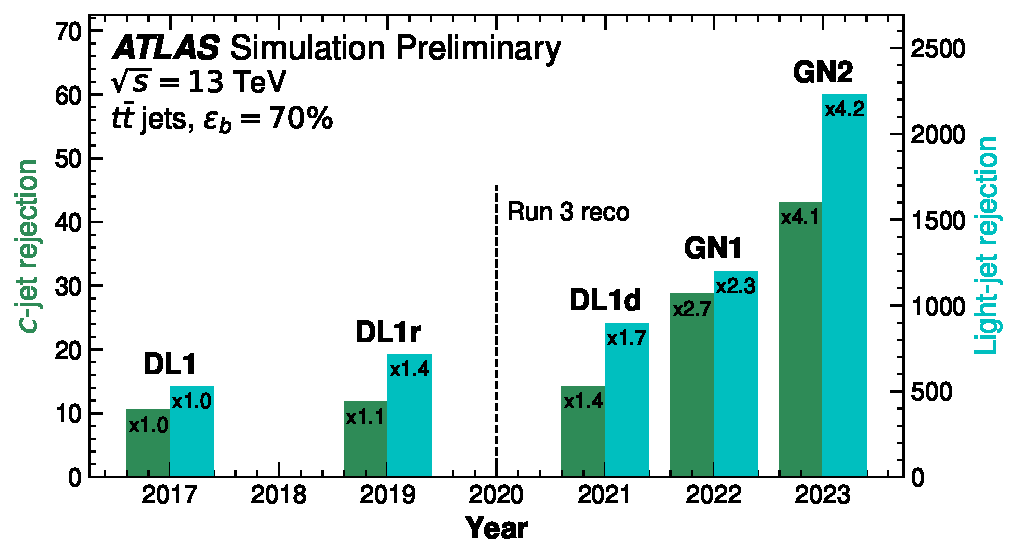
\includegraphics[width=0.6\textwidth]{figures/flavour_tagging/year_improvement.pdf}
    \caption{The $c$- and light-jet rejection of the different ATLAS flavour tagging algorithms over time in Monte Carlo simulationed jets. The rejections are provided at the 70\% $b$-tagging WP. The improvement with respect to the DL1 rejection is marked on each bar. Between DL1r and DL1d, a transition from Run 2 to Run 3 reconstruction took place. Image taken from Ref.~\cite{GN2Plots}.}
    \label{fig:ftag_better}
\end{figure}

\section{Further utilization of GN2 and Salt}

The GN2 tagger and the Salt framework have been used extensively in other analyses and areas of the collaboration.

In addition to flavour tagging, the GN2 tagger was retrained for identifying large-radius jets originating from boosted Higgs bosons decaying into $b\bar{b}$ and $c\bar{c}$ pairs~\cite{GN2X}.
In this scheme the main backgrounds are top quark pairs and multiset events.
The model, named GN2X, offered considerable classification performance over the established baselines as shown in \Cref{fig:gn2x}.

GN2 was also repurposed for constituent-based $b$-jet calibration, whereby the model was trained to regress correction factors for the jet kinematics~\cite{GN2Calib} and initial results are shown in \Cref{fig:gn2calib}.
Outside even jets, the model and Salt framework is now a part of several ongoing projects within the ATLAS including e/gamma calibration, pileup rejection, multi-top analyses, and lepton tagging.

\begin{figure}
    \centering
    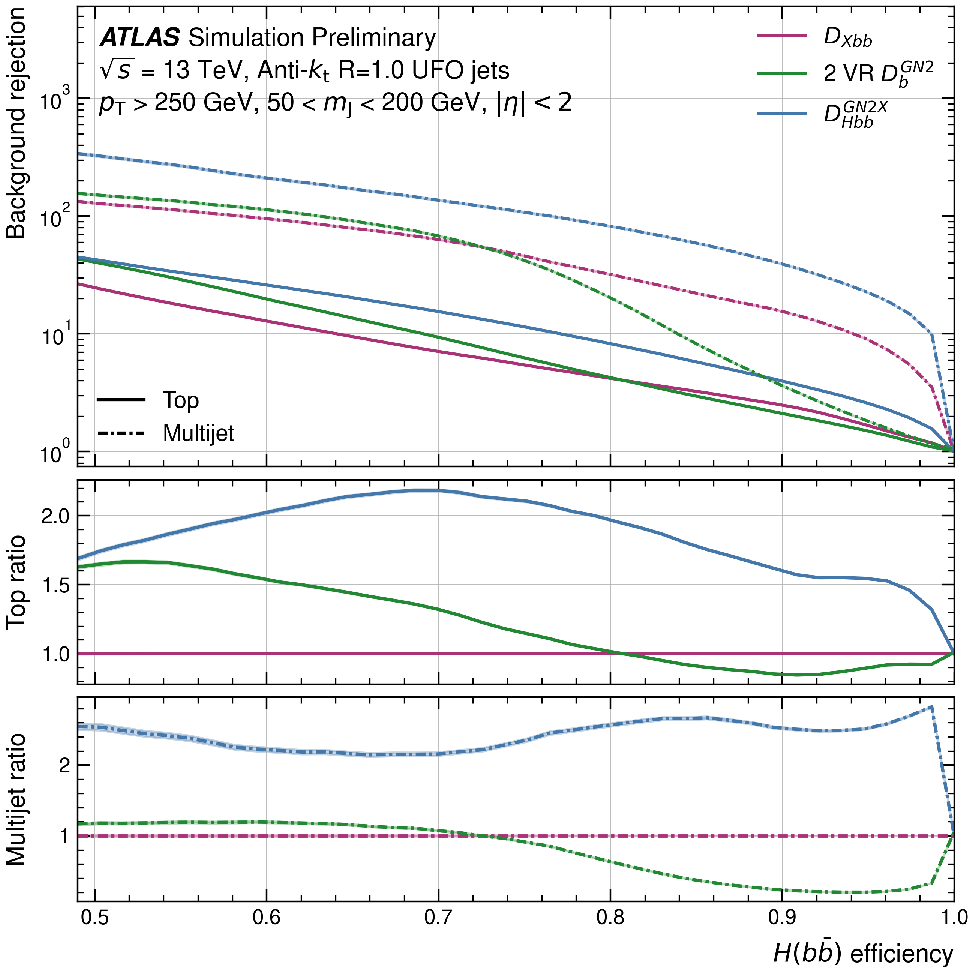
\includegraphics[width=0.49\textwidth]{figures/flavour_tagging/gn2x.pdf}
    \caption{ROC curves for $H(b\bar{b})$ tagging against top and multi-jet backgrounds for jets with $\pt>250~\GeV$ and $50<m<200~\GeV$. Performance of the GN2X algorithm is compared to the $D_{Xbb}$ and VR subjet baselines. Error bands are derived from binomial uncertainties. Plot taken from Ref.~\cite{GN2X}.}
    \label{fig:gn2x}
\end{figure}

\begin{figure}
    \centering
    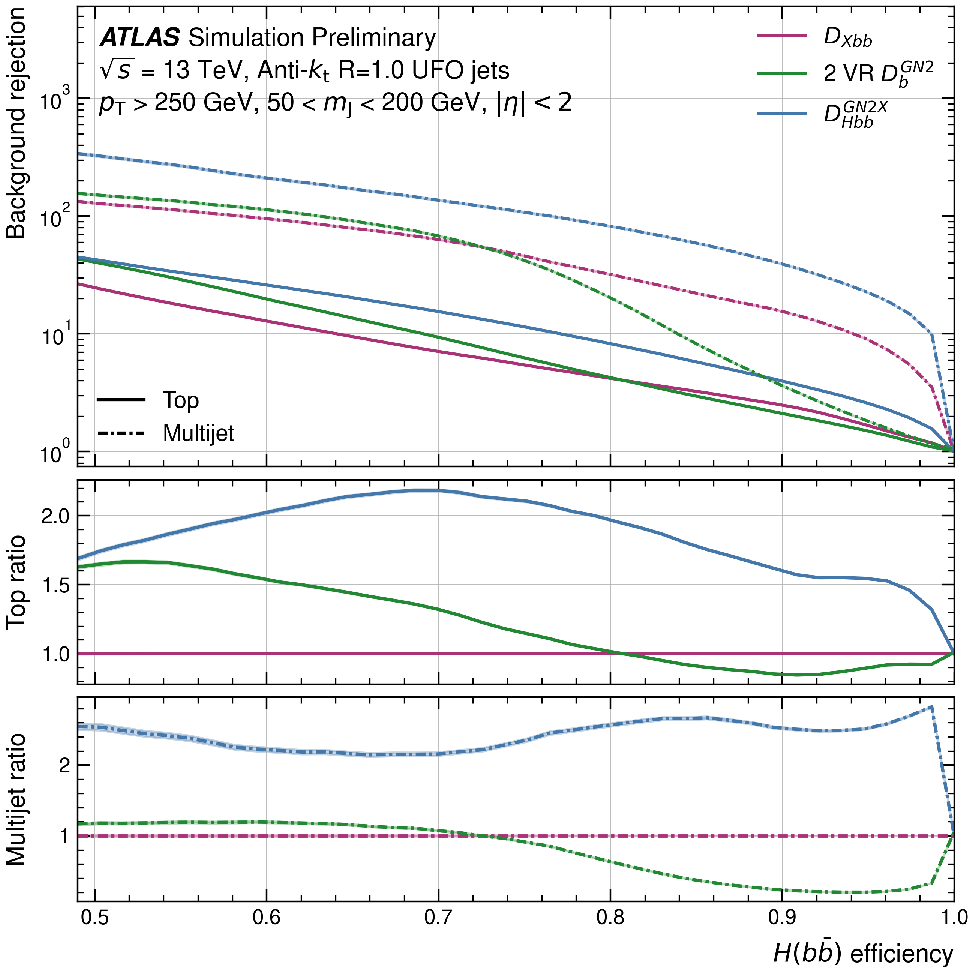
\includegraphics[width=0.49\textwidth]{figures/flavour_tagging/gn2x.pdf}
    \caption{ROC curves for $H(b\bar{b})$ tagging against top and multi-jet backgrounds for jets with $\pt>250~\GeV$ and $50<m<200~\GeV$. Performance of the GN2X algorithm is compared to the $D_{Xbb}$ and VR subjet baselines. Error bands are derived from binomial uncertainties. Plot taken from Ref.~\cite{GN2X}.}
    \label{fig:gn2x}
\end{figure}

\subsection{Future Work}

There are a number of avenues for future work that could be explored to further improve the performance of the models.

As of writing research and development in the latest iteration of the tagger GN3 is ongoing.
This model includes contributions from neutral and charge particle flow objects, as opposed to being entirely track based.
Early results indicate that this increases the tagger performance.
However, the multiplicity of the input set also increases to around 120, meaning significant work is being done behind the scenes to optimize computational performance to handle this increase in complexity, such as the incorporation of flash-attention~\cite{FlashAttentionFastMemoryEfficient}.

Another possible improvement to the model a reframing of the auxiliary tasks.
The vertexing task is largely unchanged from GN1, which itself was based on the work by~\textcite{SecondaryVertexFinding}.
In this task all pairs of output embeddings are concatenated (with both permutations) and passed through an MLP to predict the vertex label.
However, since moving to the transformer architecture, it might be worth utilizing the attention mechanism to perform this task.
Storing and updating the attention mechanism from each layer provides the required $N^2$ interaction matrix which could be used directly to perform this task.
This is in essence attempting to construct persistent edge information in the transformer model which proved to be so beneficial in the graph network models.
However, it would require a significant reworking of the model, and would clash with the computation improvements that have been made to the model.
For example, flash-attention operates by never manifesting the full attention matrix.

The vertexing task also has many similarities with the task of semantic segmentation in computer vision.
Both of these tasks predict the class of compositional elements within the input data.
Current state-of-the-art models for semantic segmentation use the MaskFormer model~\cite{MaskFormer} and initial work has shown that this too can be used to perform vertex fitting in jets~\cite{MaskFormerJets}.

Finally, there has been alot of work done on the design of specialised transformer-like layers that adhere to symmetries in the input data~\cite{GeometricAlgebraTransformer}.
This has been applied successfully to constructing classifiers for physics data that are invariant under the Lorentz group~\cite{LorentzEquivariantGeometricAlgebra}.
It would be interesting to see if such a model could be used for flavour tagging.
The reason why this is in question, as these models showed impressive performance when applied to input data containing particle 4 momentum.
However, the inputs to the tagger are sets of tracks and track reconstruction is not invariant under the Lorentz group.
While these models do describe a mechanism by which symmetry can be broken in the transformations, it remains to be seen if they can be applied to the ATLAS flavour tagging problem.






